\section{User Documentation}
\label{sec:userdocs}

This attachment serves as a guided tour of the game and its features.
It is written in such a way that it can be understood even by persons
without a~technical background. These persons may wish to simply
play the game without necessarily developing AI for it, and this attachment
is meant to give them the necessary knowledge.

\subsection{Requirements}

To run \emph{Colonizers}, the Windows 10 operating system is required.
Also required is the following software:
\begin{itemize}
    \item .NET Core 3.1 Runtime
    \item ASP.NET Core 3.1 Runtime
    \item Python 3.7
\end{itemize}
The game's UI is designed for a minimum screen resolution of 1920x1080 at
100\% zoom level. It is not recommended to play the game on lower resolution
screens, since graphical errors may occur.

\subsection{Installation}

\emph{Colonizers} is distributed via an installer application, which is shown
in \Cref{ud:installer}.

\begin{figure}[ht]
\centerline{\mbox{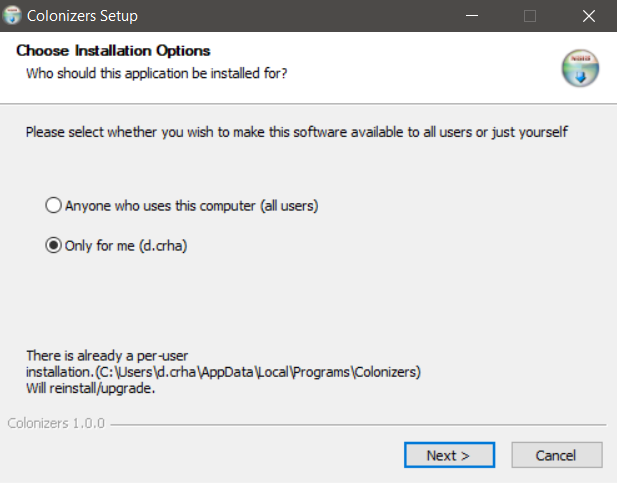
\includegraphics[width=110mm]{installer}}}
\caption{\emph{Colonizers} installer.}\label{ud:installer}
\end{figure}

The installer is an executable named \texttt{Colonizers Setup $x$.$y$.$z$.exe},
where $x$, $y$ and $z$ are placeholders for application versions. During installation,
the user will be asked whether they wish to install the application only for themselves,
or for all users of the computer. We recommend installing the application
only for the current user, since it does not require elevation. The installer
also allows the user to configure the installation directory,
as shown in \Cref{ud:installpath}.

\begin{figure}[ht]
\centerline{\mbox{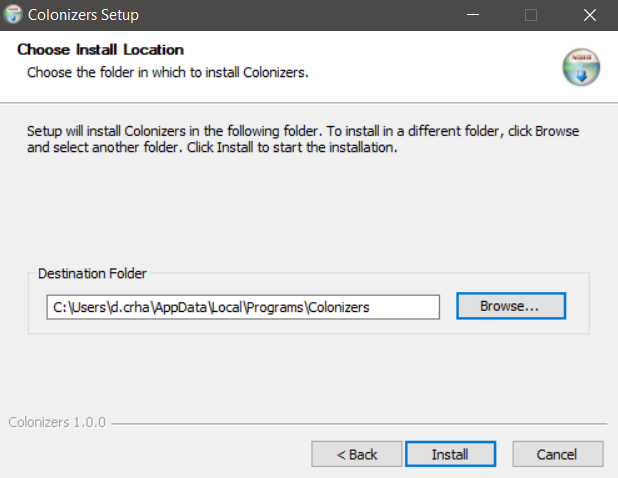
\includegraphics[width=110mm]{installpath}}}
\caption{Choosing the installation path in the installer.}\label{ud:installpath}
\end{figure}

When the installation is finished, the application may be launched from the specified
directory. The installer also adds \emph{Colonizers} into the Start menu, and creates
a~desktop shortcut for the game.

\subsection{Game Configuration}

After launching \emph{Colonizers}, the user will be presented with a~configuration
screen. On this screen, it is possible to configure the game and AI.

The first notable portion of this screen is the player selection, as shown
in \Cref{ud:playerselect}.

\begin{figure}[ht]
\centerline{\mbox{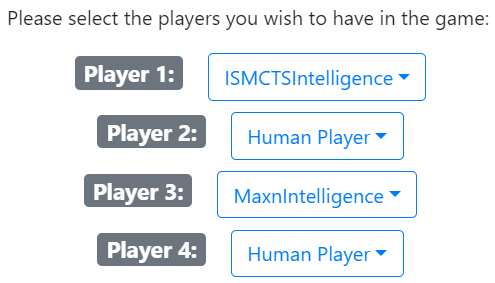
\includegraphics[width=110mm]{playerselect}}}
\caption{Player selection.}\label{ud:playerselect}
\end{figure}

This section contains four dropdowns, each
corresponding to a~player. Each dropdown lists all the available AIs
which are present in the user's game installation. By default, these dropdowns
will have the following values:
\begin{itemize}
    \item \texttt{Human Player}
    \item \texttt{HeuristicIntelligence}
    \item \texttt{ISMCTSIntelligence}
    \item \texttt{MaxnIntelligence}
    \item \texttt{RandomIntelligence}
\end{itemize}
\texttt{Human Player} means that on this player's turn, the UI will become interactible
and the user must choose action to perform. The other player options are AIs which
are bundled with the game. \Cref{ud:aicomp} shows a comparison of the aforementioned
AIs, based on the result of this thesis' experiments. Based on this table,
the user can choose the AI opponents which suit their needs.

\begin{table}[ht]
\centering
\begin{tabular}{l@{\hspace{1.5cm}} c c c c}
\textbf{AI} & \textbf{Strength} & \textbf{Evaluation speed} \\
\midrule
\texttt{RandomIntelligence}      & Weak   & Fast   \\
\texttt{HeuristicIntelligence}   & Moderate   & Fast  \\
\texttt{MaxnIntelligence}        & Moderate   & Moderate  \\
\texttt{ISMCTSIntelligence}      & Strong   & Slow   \\
\bottomrule
\end{tabular}
\caption{Simplified AI comparison.}\label{ud:aicomp}
\end{table}

There is an option to not enable information hiding. Normally, certain information
would be hidden on the screen, since that information is hidden in the game.
However, for purposes of testing AI, the option shown by \Cref{ud:hiddeninfo} can
be left unchecked. This will reveal all hidden information in the UI.
Note that this option does not affect the AI in any way, this option
is purely a~cosmetic one.

\begin{figure}[ht]
\centerline{\mbox{
\includegraphics[width=110mm]{hiddeninfo}}}
\caption{Checkbox for hiding information.}\label{ud:hiddeninfo}
\end{figure}

The next section of configuration is are the buttons for adding new AI
into the game, as shown in \Cref{ud:aiaddbuttons}.

\begin{figure}[ht]
\centerline{\mbox{
\includegraphics[width=110mm]{aiaddbuttons}}}
\caption{Buttons for adding new AI scripts.}\label{ud:aiaddbuttons}
\end{figure}

These buttons open file select dialogs, allowing the user to add new AIs.
When adding an AI script, the script must follow the naming convention
of \texttt{<Name>Intelligence.py}, for example \texttt{CleverIntelligence.py}
\footnote{If an~AI is added this way which shares a~name with and existing AI,
the existing AI will be replaced by the new one. This also applies to AIs which
are bundled with the game}.
If the selected file does not follow this convention, it will not be recognized
by the game.
When adding an AI folder, the folder must follow the naming convention of
\texttt{<Name>Intelligence}, and this folder must contain a \texttt{main.py}
script. If the folder does not follow these conventions, it will not be recognized
by the game. This is explained in more depth in \Cref{sec:aiadd}.

Lastly, this screen allows the configuration of the Python executable used
to execute AI scripts, as seen in \Cref{ud:pythonselect}. The shown
button will open a file select dialog, where the user can select their
installed Python executable.

\begin{figure}[ht]
\centerline{\mbox{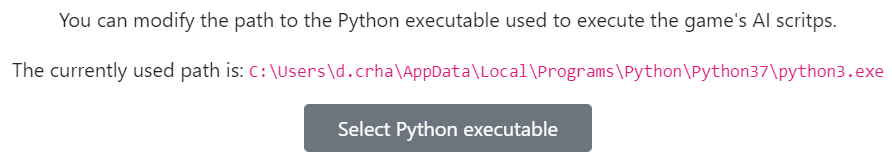
\includegraphics[width=110mm]{pythonselect}}}
\caption{Configuration of Python executable.}\label{ud:pythonselect}
\end{figure}

After the user is done configuring the game, they may start a game by clicking the
\emph{START GAME} button. Note that this button is disabled if the user
has not specified a Python executable to use.

\subsection{Gameplay}

If the reader has not yet read \Cref{chap:gamerules} before reading this section,
it may be wise to do so now, in order for them to be familiar with
the game's rules.

\subsubsection{Board Overview}

After launching the game, the user will be greeted with a~view similar to
the one depicted in \Cref{ud:overview}.

\begin{figure}[ht]
\centerline{\mbox{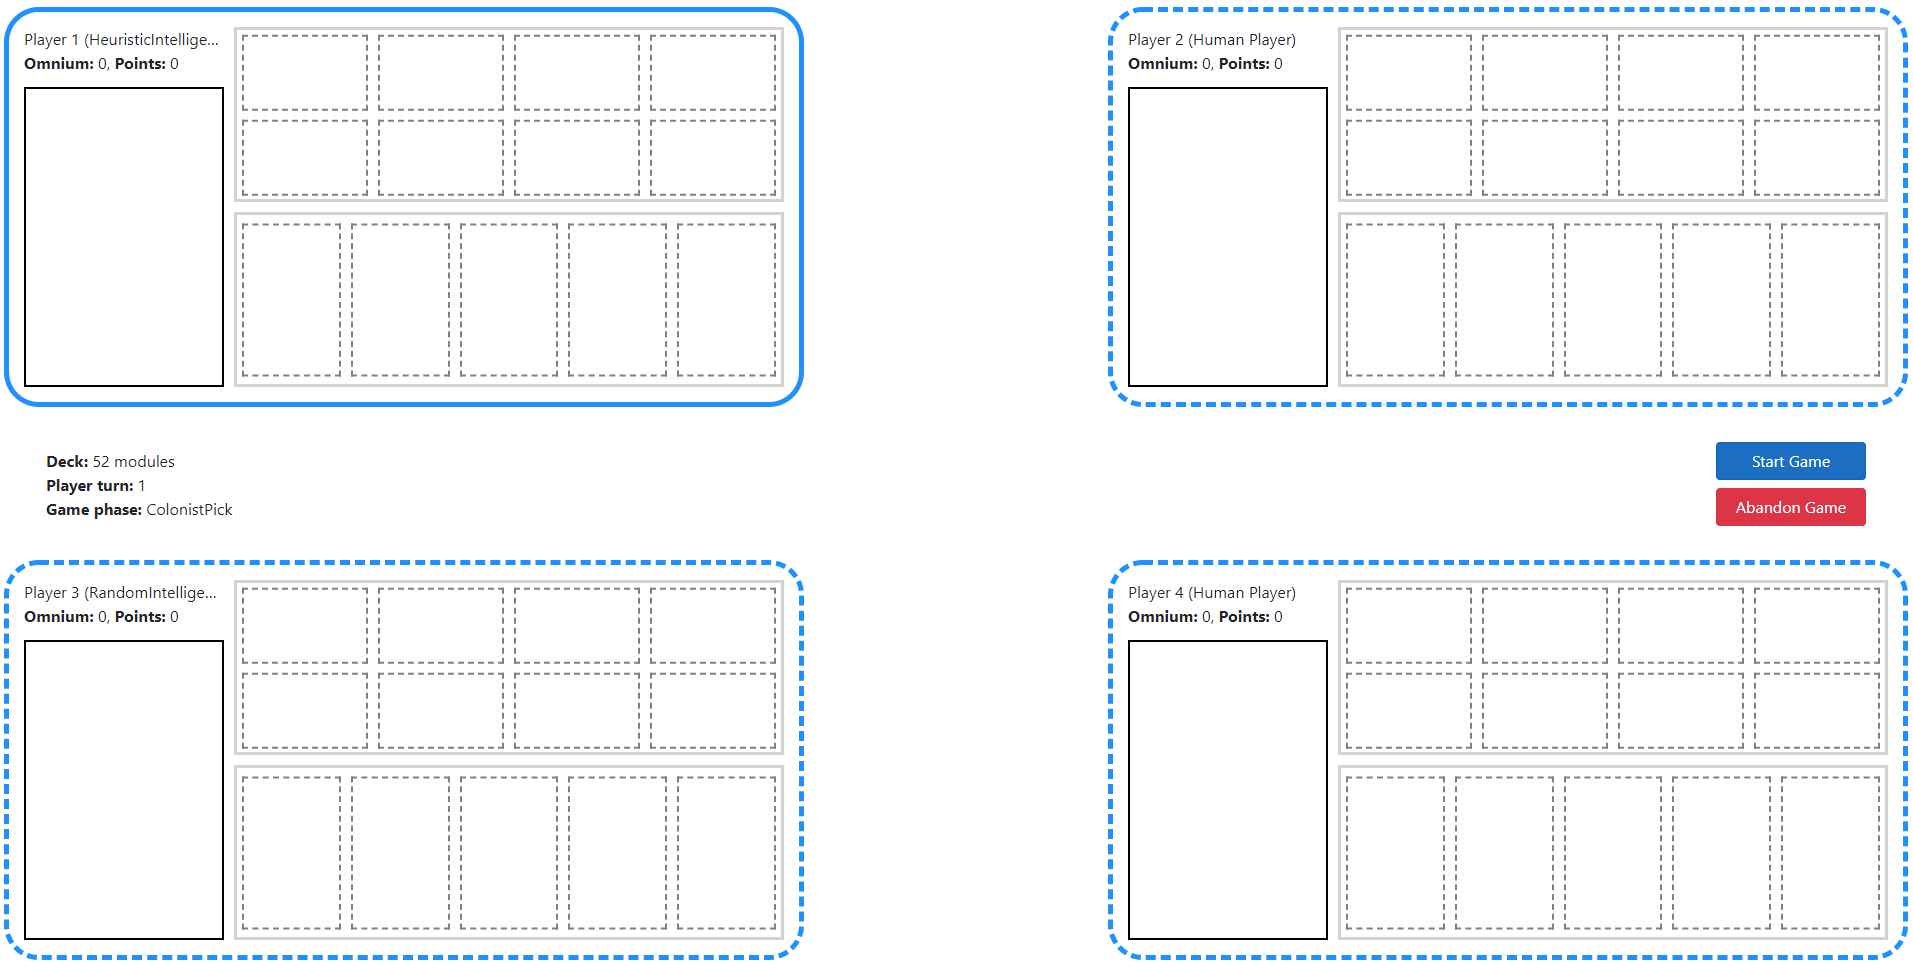
\includegraphics[width=130mm]{overview}}}
\caption{Overview of main game screen.}\label{ud:overview}
\end{figure}

This is the main game screen, and it is where all gameplay will be happening.
First off, we can focus on the buttons to the right of the screen, as shown in
\Cref{ud:buttons}.

\begin{figure}[ht]
\centerline{\mbox{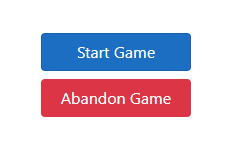
\includegraphics[width=60mm]{buttons}}}
\caption{Game control buttons.}\label{ud:buttons}
\end{figure}

These buttons control the flow of the game. The game does not start until the user
presses the \emph{Start Game} button. When the user does press it, the game starts
and the buttons becomes disabled. The other button, \emph{Abandon Game}, may be
pressed at any time during gameplay to immediately end the current game and return
to the configuration screen.

On the left side of the screen, we can also see miscellaneous information about the
game state written in plain text. This information includes the amount of modules
left in the deck, the player on turn, and the current game phase.

The player overview areas are a core part of gameplay, you can see an example
of this area in \Cref{ud:player}.

\begin{figure}[ht]
\centerline{\mbox{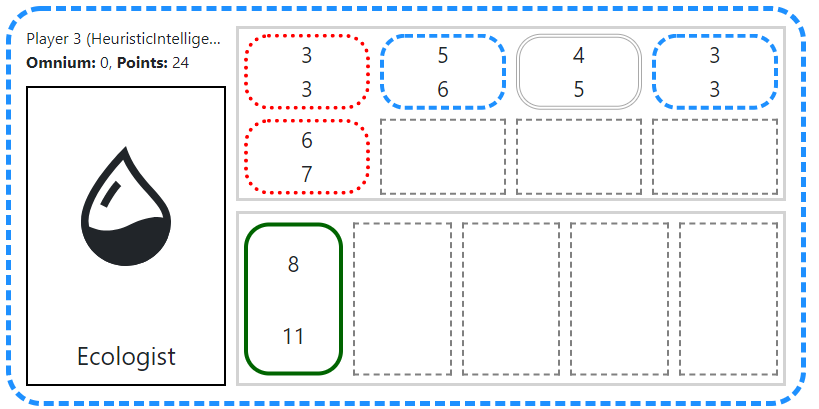
\includegraphics[width=110mm]{player}}}
\caption{Player overview.}\label{ud:player}
\end{figure}

This area contains all information about a given player. In the top left,
it shows the player's position and their name (meaning either \emph{Human Player},
or the name of the AI playing this player). In the top left we can also see
the amount of Omnium the player has (the game's currency) and the number of points
the player has the number of points determines the ranking at the end of the game.

On the left side of the player overview is the player's colonist card. This shows
the colonist this player has selected. A~colonist is a~character controlled
by the player for a~single turn, and the colonist provides the player with
special abilities to use at specific times of the game. The colonist is
easily identifiable by the icon and large text below it. For a~full description
of what abilities colonists have, please refer to \Cref{gamedesign:colonists}.

It is possible for this colonist card to be hidden, instead displaying a~card
featuring a large question mark. This can happen when hidden information is enabled
during game configuration. Specifically, a~player can only see another player's
colonist if the other player has already taken their turn.

Another feature shown by \Cref{ud:player} is the colony overview, seen in
\Cref{ud:colony}. This area contains the modules the player has built during
the game. The colony area has eight possible slots to build on. A square with
a grey dashed border is an empty slot. When any player
builds eight modules in their colony, the game will end at the end of the round,
after all players have taken their turn.

\begin{figure}[ht]
\centerline{\mbox{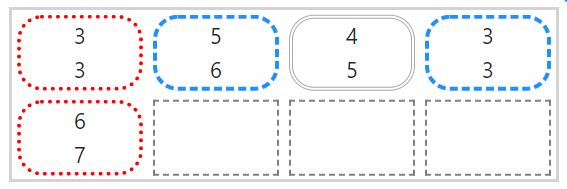
\includegraphics[width=110mm]{colony}}}
\caption{The colony overview.}\label{ud:colony}
\end{figure}

The elements with colored borders and two numbers inside them are called modules.
They are drawn by players from the deck, and they can be built in a~player's colony.
In order to build a module, the player must pay its build cost. A~module's build cost
is the number shown in the upper part of the module. When build in a~player's colony,
modules count towards that player's score. A~module's contribution to a player's
score is the number found in the bottom part of the module. Modules also have
a~color, depicted by the colored border \footnote{In order for the game to be accessible
to colorblind persons, the borders are also distinguished by the border pattern. A solid
line means green, a dashed line means blue, a dotted line means red, and a double line means
a module without a color.}
. This color is relevant during interactions
with certain colonist abilities. The modules in a player's colony are not hidden, and
are visible to other players even when information hiding is enabled.

The player overview seen in \Cref{ud:player} also contains the player's hand, as seen
in \Cref{ud:hand}.

\begin{figure}[ht]
\centerline{\mbox{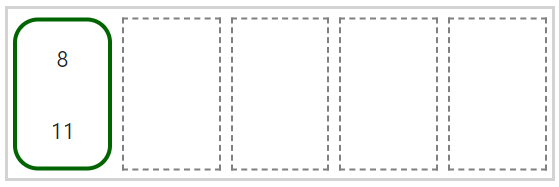
\includegraphics[width=110mm]{playerhand}}}
\caption{A player's hand.}\label{ud:hand}
\end{figure}

Whenever a player draws modules from the deck, they go into their hand. They then remain in
their hand until they are built, or removed by other means. The hand has a size limit of
five, it is not possible to draw more modules when a~player is at five modules in hand.
The modules in other players' hands are among the parts of the game board affected
by information hiding. If information hiding is enabled, modules in the hands of other
players will be displayed without color, and with question marks instead of
their real values.

The last feature of the player overview is its blue border. In \Cref{ud:player},
this border is dashed, meaning it is currently another player's turn. The player on
turn always has a~solid border around their player overview.

\subsubsection{Taking Turns}

Firstly, it should be noted that AIs take turns autonomously without any need of input
from the user. Whenever the turn is passed to an AI, it will immediately start
looking for the best move, and as soon as that move is found, it is played and the game
continues. This means that with AIs that make decisions particularly fast, if the game
is configured to have four of these AIs, the game can potentially end in mere seconds.
Therefore we will be discussing only features related to human players taking turns
for the rest of this section.

The first phase of a turn is the colonist pick phase. If you set up a game where
the first position has a human player, you will immediately be greeted with a selection
similar to the one seen in \Cref{ud:colonistpick}.

\begin{figure}[ht]
\centerline{\mbox{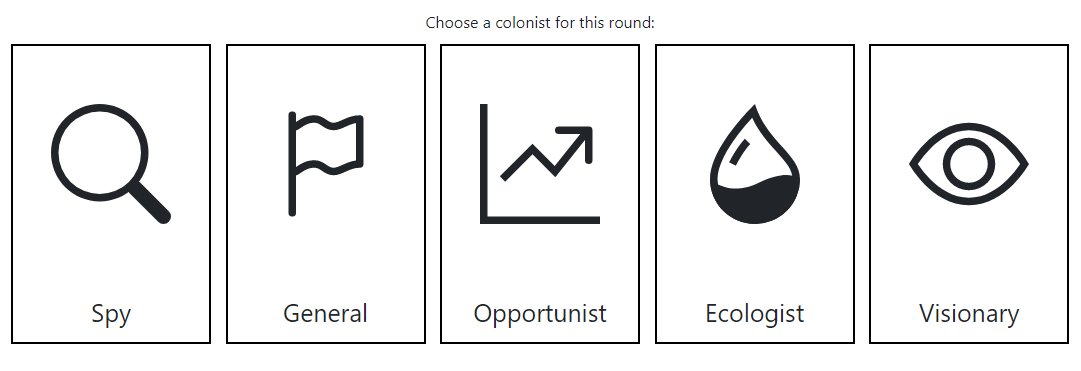
\includegraphics[width=130mm]{colonistpick}}}
\caption{Colonist selection.}\label{ud:colonistpick}
\end{figure}

At the start of each round, all players will take turns picking a colonist,
in order of first player to last. Note that only five out of the total
six are available for selection at any given time, since one is randomly removed
from play every round. Selecting a colonist is done by clicking on the corresponding
colonist card.

After all players have picked their colonist, players will each take their turn,
in order from first to last. The first phase of a player's individual turn is
the draw phase, as seen in \Cref{ud:drawphase}. The shown buttons will be present
in a card overlaying the game board, similarly to the colonist pick phase.
Colonist passive abilities trigger automatically during the draw phase.

\begin{figure}[ht]
\centerline{\mbox{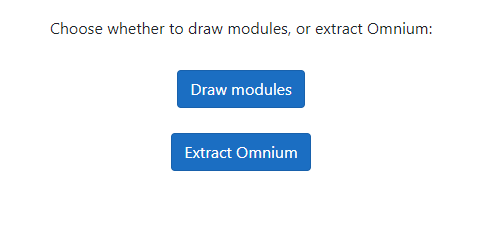
\includegraphics[width=110mm]{drawphase}}}
\caption{Draw phase selection.}\label{ud:drawphase}
\end{figure}

At this point, a player may choose to either gain two Omnium, order
draw two modules from the deck and discard one of them.
Note that the draw action will be unavailable if the player's hand is full.
If the player chooses to draw modules, they will be presented with an additional
dialog as seen in \Cref{ud:discardphase}. The player must choose which module they
want to keep, and which they want to discard. The choice is made by clicking on the
module the player wishes to keep.

\begin{figure}[ht]
\centerline{\mbox{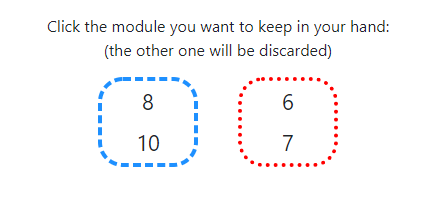
\includegraphics[width=110mm]{discardphase}}}
\caption{Choice of module to discard.}\label{ud:discardphase}
\end{figure}

The next phase is the colonist power phase. If the player control a~colonist
with an~active ability (Opportunist or Spy), they will be presented with a~choice
similar to that shown in \Cref{ud:powertarget}. The player may choose to target
a given colonist by clicking on their respective card, or the player may choose
to not use their colonist's ability by clicking the \emph{Do nothing} button
to the right.

\begin{figure}[ht]
\centerline{\mbox{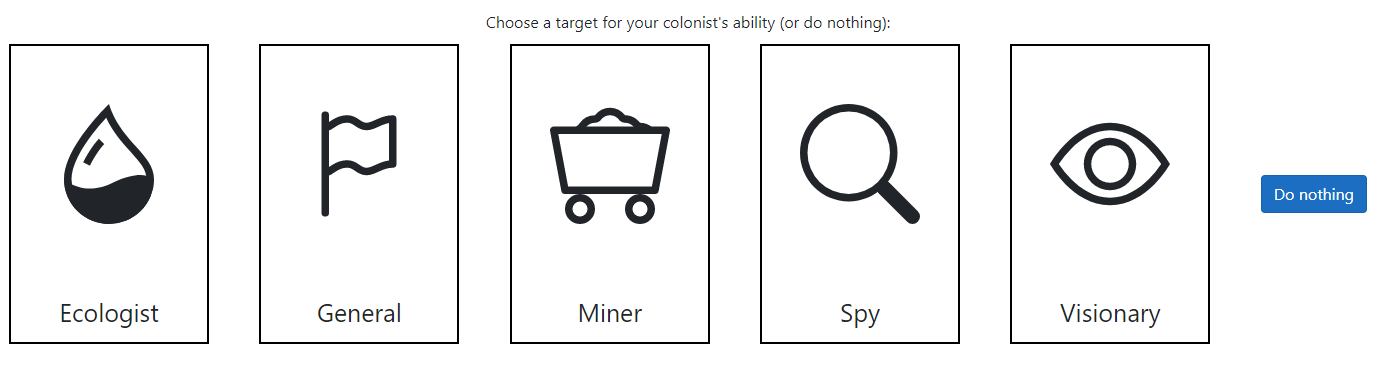
\includegraphics[width=130mm]{powertarget}}}
\caption{Selection of colonist active ability target.}\label{ud:powertarget}
\end{figure}

Players controlling colonists without active abilities will instead be presented
with a small dialog containing a single button which passes the phase.

The last phase of a turn is the build phase. In this phase, players may build
up to one module from their hand by spending the required amount of Omnium.
Modules which the player can afford to build will have a hammer icon present.
Clicking this icon will build the module in the player's colony. If the hammer
icon is not present, it means that the player cannot afford the module,
or the game is not in the build phase. The hammer icon is shown in
\Cref{ud:buildhammer}, next to a module without the hammer icon.

\begin{figure}[ht]
\centerline{\mbox{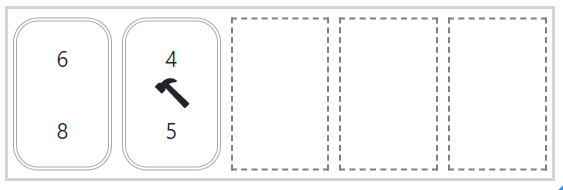
\includegraphics[width=110mm]{buildhammer}}}
\caption{Hammer icon used to build modules from the hand.}\label{ud:buildhammer}
\end{figure}

After all players end their turns, the round will end and a new round will begin,
starting again with the colonist pick phase. New rounds will keep
starting after the previous round ends until a player has built eight
modules in their colony. The first player to reach eight modules receives
four bonus point on game end, and subsequent players to reach eight modules
receive two points each. When the game ends, a dialog will open showing the user
the final ranking and final scores. This final score table is shown in
\Cref{ud:gameover}.

\begin{figure}[ht]
\centerline{\mbox{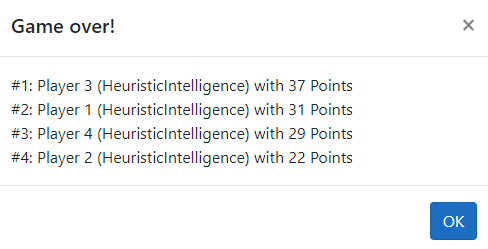
\includegraphics[width=110mm]{gameover}}}
\caption{Game over screen with final scores.}\label{ud:gameover}
\end{figure}

Here, the player may either click \emph{OK} to go back to the game configuration
screen, or they may simply close the dialog and spend time looking at the final
game board state. When the user wishes to return to the game configuration screen,
they may press the \emph{Abandon Game} button to do so.

\clearpage
